\begin{figure}

\includegraphics[width=0.4\linewidth]{linuxreader-img028.png}
	\caption{Het zoeken van informatie}
\end{figure}

Om uit te vinden welk commando je kan gebruiken om iets op het systeem te bereiken kan je man -k gebruiken. Een
alternatief commando is apropos. Type eens:

\begin{lstlisting}[language=bash]
$ apropos `make directories'
\end{lstlisting}
je vindt dan het `mkdir' commando. Het nadeel van dit zoek systeem is dat het redelijk specifiek is.

\begin{lstlisting}[language=bash]
$ apropos `make directory'
\end{lstlisting}
doet niets. Als je het dus niet meteen vindt probeer dan enkelvoud- en meervoudsvormen.

Heb je een commando gevonden waarvan je denkt dat het is wat je nodig hebt probeer dan man -f of whatis.

\begin{lstlisting}[language=bash]
$ whatis mkdir
\end{lstlisting}

Dit geeft een korte beschrijving van een commando en voor de volledige manual gebruiken we het man commando:
\begin{lstlisting}[language=bash]
$ man mkdir
\end{lstlisting}

Extra uitleg van een commando kan vaak ook gevonden worden door -h of --help aan het commando toe te voegen met een
spatie.

\begin{figure}[H]
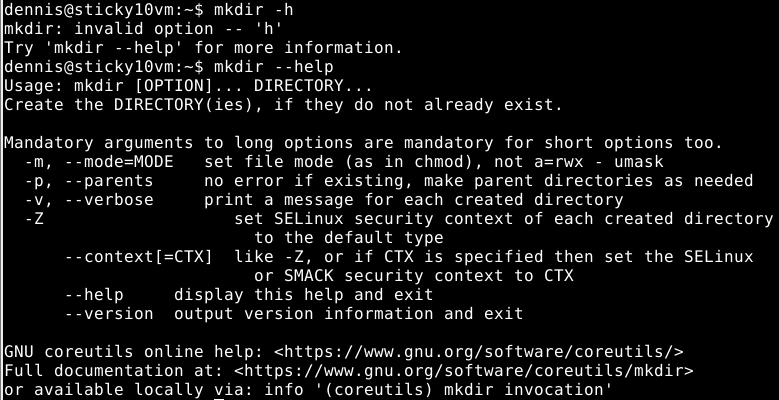
\includegraphics[width=0.8\linewidth]{linuxreader-img029.png}
	\label{fig:DocHelp}
	\caption{Gebruik van -h of --help}
\end{figure}

Zoals je ziet in \ref{fig:DocHelp} dat -h een error melding geeft en ons vertelt dat we -{}-help moeten gebruiken. Ook wordt er verteld wat we de
volledige documentatie online kunnen vinden in de info-documentatie.

